\documentclass[aspectratio=169,11pt]{beamer}
\usepackage[T1]{fontenc}
\usepackage{lmodern,amsmath,amssymb,mathtools,bm,booktabs,array,graphicx,tikz}
\usetikzlibrary{arrows.meta,positioning,calc,decorations.pathreplacing,patterns}
\definecolor{ink}{HTML}{17344D}\definecolor{accent}{HTML}{087E8B}\definecolor{pale}{HTML}{EDF5F5}\definecolor{gold}{HTML}{AD6B19}
\providecommand{\dd}{\,\mathrm{d}}\providecommand{\R}{\mathbb{R}}
\providecommand{\E}{\mathbb{E}}\providecommand{\Var}{\operatorname{Var}}
\providecommand{\Cov}{\operatorname{Cov}}\providecommand{\diag}{\operatorname{diag}}
\providecommand{\norm}[1]{\left\lVert#1\right\rVert}
\providecommand{\abs}[1]{\left|#1\right|}
\usefonttheme{professionalfonts}
\setbeamercolor{normal text}{fg=black,bg=white}
\setbeamercolor{frametitle}{fg=ink,bg=white}
\setbeamercolor{title}{fg=ink}\setbeamercolor{structure}{fg=accent}
\setbeamercolor{block title}{fg=ink,bg=pale}\setbeamercolor{block body}{fg=black,bg=pale!40}
\setbeamercolor{alerted text}{fg=accent}
\setbeamerfont{frametitle}{size=\Large,series=\bfseries}
\setbeamerfont{title}{size=\LARGE,series=\bfseries}
\setbeamertemplate{navigation symbols}{}
\setbeamersize{text margin left=.7cm,text margin right=.7cm}
\setbeamertemplate{frametitle}{\vspace{.18cm}\insertframetitle\par\vspace{.1cm}{\color{accent}\hrule height .6pt}\vspace{.12cm}}
\newcommand{\notestarget}{notes.pdf}\newcommand{\noteslabel}{Notes}
\setbeamertemplate{footline}{\hspace{.7cm}\color{ink}\scriptsize Computational Cardiology\quad\href{\notestarget}{\noteslabel}\hfill\insertframenumber\,/\,\inserttotalframenumber\hspace{.7cm}\vspace{.18cm}}
\setbeamercovered{invisible}
\hypersetup{pdfauthor={Zan Ahmad},pdftitle={Surrogate error, amortized cost and training-step bias},pdfpagemode=UseNone}
\begin{document}
\begin{frame}[plain]\vfill
{\small\color{accent} Computational Cardiology \quad Lecture 19}\par\medskip
{\raggedright\hyphenpenalty=10000\exhyphenpenalty=10000\LARGE\bfseries\color{ink} Surrogate error, amortized cost and training-step bias}\par\bigskip
Zan Ahmad\par\smallskip
{\small Fall 2024}\par\vfill\end{frame}
\renewcommand{\notestarget}{notes.pdf\#note-reference-error-and-approximation-error}
\begin{frame}[t,fragile,label=slide-three-solutions-in-an-error-budget]{Three solutions in an error budget}
\[\|u_{sur}-u\|\le\|u_{sur}-u_{ref}\|+\|u_{ref}-u\|.\]\pause{} Surrogate agreement and reference accuracy are separate terms.
\end{frame}
\renewcommand{\notestarget}{notes.pdf\#note-reference-error-and-approximation-error}
\begin{frame}[t,fragile,label=slide-compatibility-of-the-comparison]{Compatibility of the comparison}
The same field, physical time, coordinate representation and norm must be used.\pause{} The bound does not estimate disagreement with biological observations.
\end{frame}
\renewcommand{\notestarget}{notes.pdf\#note-amortized-computational-cost}
\begin{frame}[t,fragile,label=slide-total-reference-cost]{Total reference cost}
\[C_{ref}(Q)=QC_r.\]\pause{} $Q$ counts comparable queries under a declared timing boundary.
\end{frame}
\renewcommand{\notestarget}{notes.pdf\#note-amortized-computational-cost}
\begin{frame}[t,fragile,label=slide-total-surrogate-cost]{Total surrogate cost}
\[C_{sur}(Q)=C_0+QC_s.\]\pause{} Setup can include labels, preprocessing, spectral bases, fitting and model selection.
\end{frame}
\renewcommand{\notestarget}{notes.pdf\#note-amortized-computational-cost}
\begin{frame}[t,fragile,label=slide-strict-break-even]{Strict break-even}
\[Q>\frac{C_0}{C_r-C_s},\qquad C_r>C_s.\]\pause{} The first strictly cheaper integer count is the floor of this ratio plus one.
\end{frame}
\renewcommand{\notestarget}{notes.pdf\#note-amortized-computational-cost}
\begin{frame}[t,fragile,label=slide-geometry-dependent-setup]{Geometry-dependent setup}
A basis constructed for each geometry is a recurring cost when geometries change.\pause{} Treating it as one universal setup changes the workload being compared.
\end{frame}
\renewcommand{\notestarget}{notes.pdf\#note-matched-timing-and-accuracy-comparisons}
\begin{frame}[label=slide-a-cost-error-comparison-panel-1]{Measured CPU cost}
\centering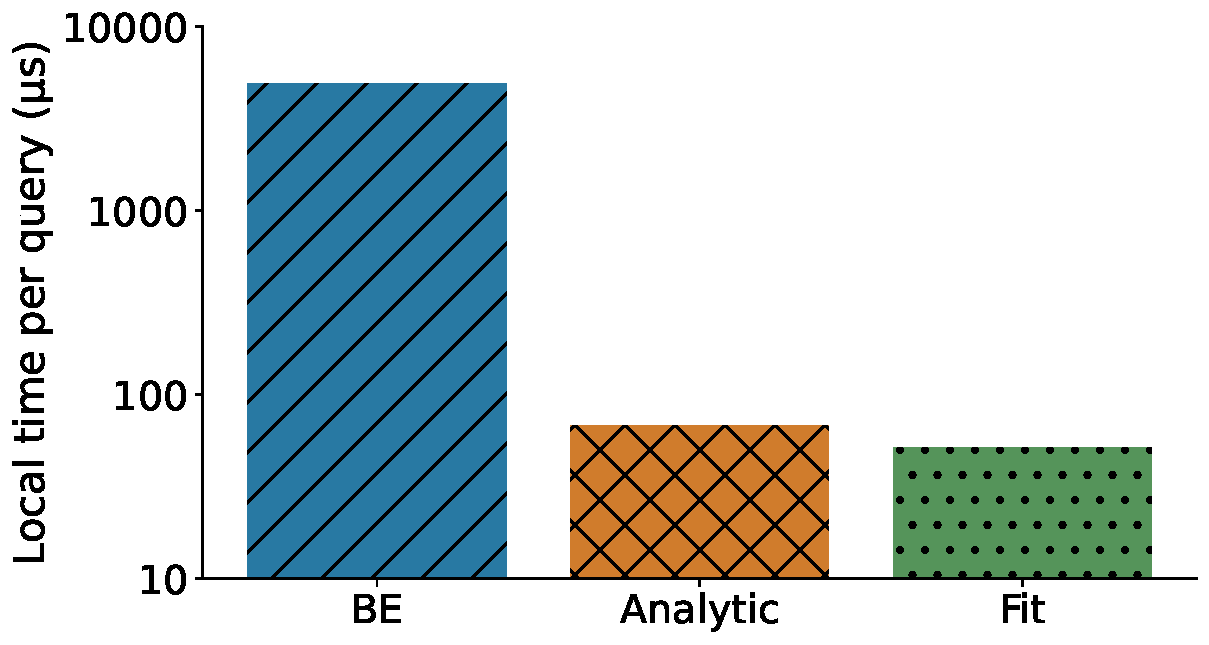
\includegraphics[width=.98\linewidth,height=.69\textheight,keepaspectratio]{presentation-figures/cost-error-panel-1.pdf}\end{frame}
\renewcommand{\notestarget}{notes.pdf\#note-matched-timing-and-accuracy-comparisons}
\begin{frame}[label=slide-a-cost-error-comparison-panel-2]{Error against analytic truth}
\centering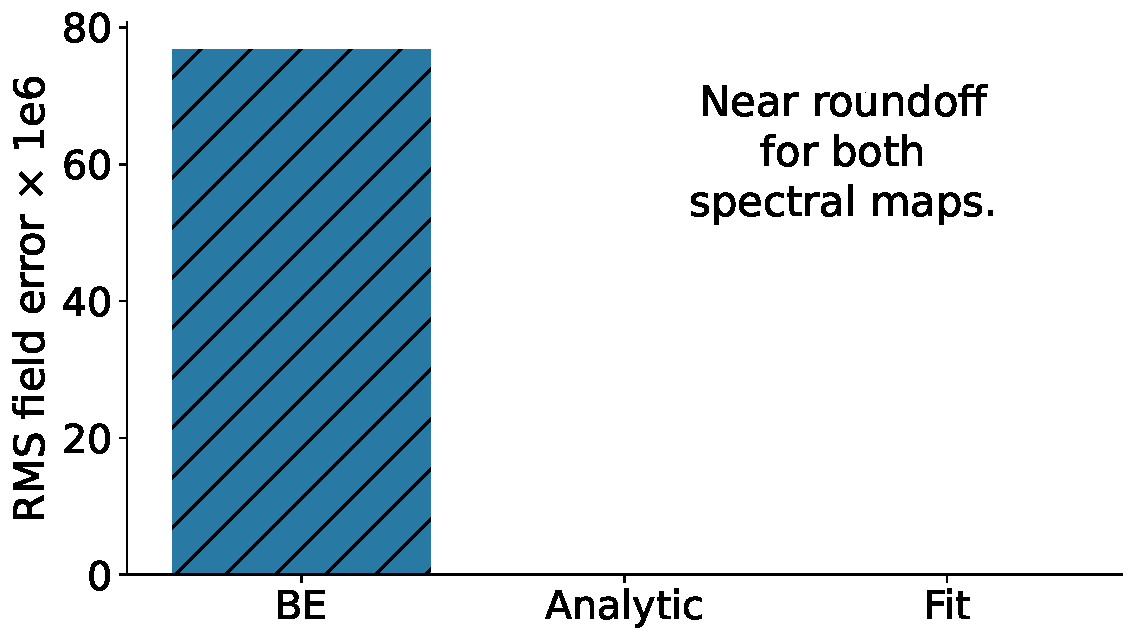
\includegraphics[width=.98\linewidth,height=.69\textheight,keepaspectratio]{presentation-figures/cost-error-panel-2.pdf}\end{frame}
\renewcommand{\notestarget}{notes.pdf\#note-matched-timing-and-accuracy-comparisons}
\begin{frame}[t,fragile,label=slide-a-cost-error-comparison]{A cost--error comparison}
Compare admissible pairs $(C,E)$ rather than cost alone.\pause{} On the heat fixture, analytic spectral evolution is a competing baseline.
\end{frame}
\renewcommand{\notestarget}{notes.pdf\#note-a-generator-fitted-through-an-euler-update}
\begin{frame}[t,fragile,label=slide-the-exact-scalar-flow]{The exact scalar flow}
\[y_t=-\lambda y,\qquad y(t+\Delta)=e^{-\lambda\Delta}y(t).\]\pause{} Take $y(0)=1$ for the numerical example.
\end{frame}
\renewcommand{\notestarget}{notes.pdf\#note-a-generator-fitted-through-an-euler-update}
\begin{frame}[t,fragile,label=slide-fit-a-generator-through-forward-euler]{Fit a generator through forward Euler}
\[y^{n+1}=(1+\Delta a_\Delta)y^n.\]\pause{} Matching exact data gives\[a_\Delta=\frac{e^{-\lambda\Delta}-1}{\Delta}.\]
\end{frame}
\renewcommand{\notestarget}{notes.pdf\#note-a-generator-fitted-through-an-euler-update}
\begin{frame}[t,fragile,label=slide-the-fitted-rate-differs-from-the-true-rate]{The fitted rate differs from the true rate}
\[a_\Delta=-\lambda+\frac{\lambda^2}{2}\Delta+O(\Delta^2).\]\pause{} A finite training step is encoded in the fitted generator.
\end{frame}
\renewcommand{\notestarget}{notes.pdf\#note-a-generator-fitted-through-an-euler-update}
\begin{frame}[t,fragile,label=slide-exact-sampled-agreement-at-the-training-step]{Exact sampled agreement at the training step}
\[(1+\Delta a_\Delta)^n=e^{-\lambda n\Delta}.\]\pause{} This identity follows from the matching construction, not from recovering $-\lambda$.
\end{frame}
\renewcommand{\notestarget}{notes.pdf\#note-training-resolution-and-inference-resolution}
\begin{frame}[label=slide-refine-inference-while-holding-the-fit-fixed-panel-1]{A step-coupled fitted generator}
\centering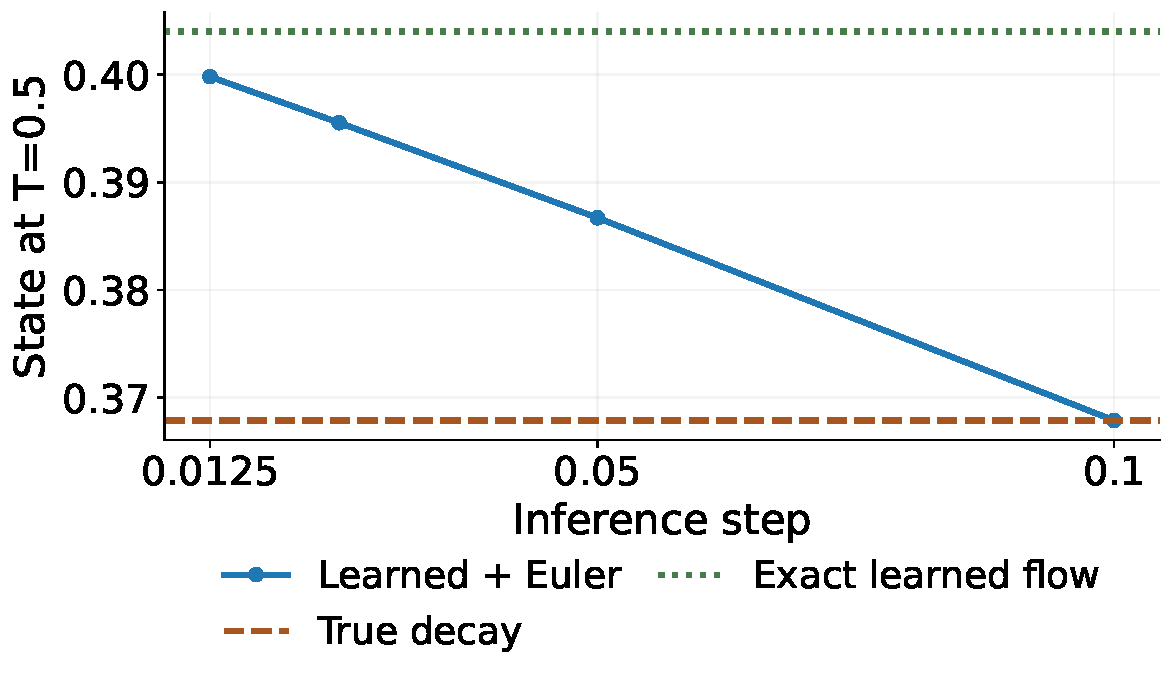
\includegraphics[width=.98\linewidth,height=.69\textheight,keepaspectratio]{presentation-figures/learned-step-panel-1.pdf}\end{frame}
\renewcommand{\notestarget}{notes.pdf\#note-training-resolution-and-inference-resolution}
\begin{frame}[label=slide-refine-inference-while-holding-the-fit-fixed-panel-2]{Smaller steps need not help}
\centering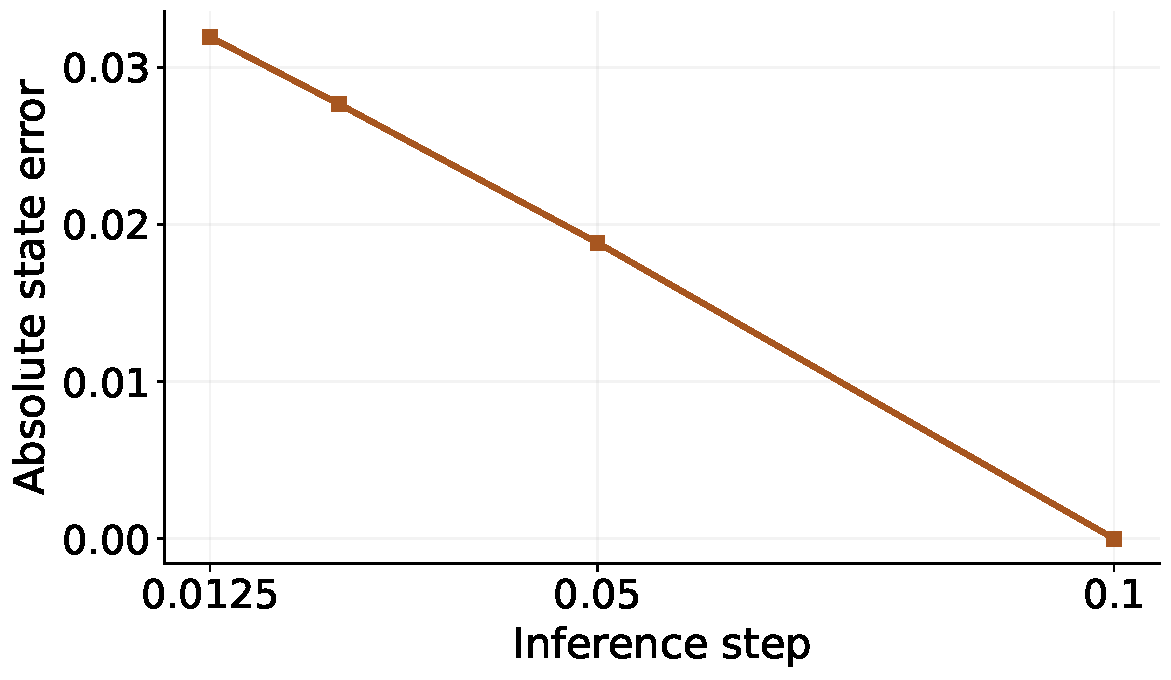
\includegraphics[width=.98\linewidth,height=.69\textheight,keepaspectratio]{presentation-figures/learned-step-panel-2.pdf}\end{frame}
\renewcommand{\notestarget}{notes.pdf\#note-training-resolution-and-inference-resolution}
\begin{frame}[t,fragile,label=slide-refine-inference-while-holding-the-fit-fixed]{Refine inference while holding the fit fixed}
\[(1+ha_\Delta)^{T/h}\longrightarrow e^{Ta_\Delta}\quad(h\to0).\]\pause{} The limit solves the learned equation more accurately.
\end{frame}
\renewcommand{\notestarget}{notes.pdf\#note-training-resolution-and-inference-resolution}
\begin{frame}[t,fragile,label=slide-a-nonvanishing-limiting-bias]{A nonvanishing limiting bias}
For $\lambda=2$, $\Delta=.1$, $T=.5$,\[e^{Ta_\Delta}\approx.403998,\qquad e^{-\lambda T}\approx.367879.\]\pause{} A smaller inference step need not reduce error to the true equation.
\end{frame}
\renewcommand{\notestarget}{notes.pdf\#note-training-resolution-and-inference-resolution}
\begin{frame}[t,fragile,label=slide-two-distinct-refinement-limits]{Two distinct refinement limits}
\[h\to0\quad\text{at fixed }\Delta\qquad\text{versus}\qquad\Delta\to0.\]\pause{} The first refines integration; the second changes the fitted generator.
\end{frame}
\renewcommand{\notestarget}{notes.pdf\#note-the-domain-of-a-computational-replacement-claim}
\begin{frame}[t,fragile,label=slide-an-admissible-computational-replacement]{An admissible computational replacement}
The surrogate must meet the stated error tolerance over the intended input regime and query workload.\pause{} Lower per-query cost alone does not establish that claim.
\end{frame}
\end{document}
